\documentclass[10pt,twocolumn,letterpaper]{article}
\usepackage[rebuttal]{cvpr}

% Include other packages here, before hyperref.
\usepackage{graphicx}
\usepackage{amsmath}
\usepackage{amssymb}
\usepackage{booktabs}
\usepackage{pdflscape}
\usepackage{float}

% If you comment hyperref and then uncomment it, you should delete
% egpaper.aux before re-running latex.  (Or just hit 'q' on the first latex
% run, let it finish, and you should be clear).
\usepackage[pagebackref,breaklinks,colorlinks,bookmarks=false]{hyperref}

% Support for easy cross-referencing
\usepackage[capitalize]{cleveref}
\crefname{section}{Sec.}{Secs.}
\Crefname{section}{Section}{Sections}
\Crefname{table}{Table}{Tables}
\crefname{table}{Tab.}{Tabs.}

% If you wish to avoid re-using figure, table, and equation numbers from
% the main paper, please uncomment the following and change the numbers
% appropriately.
%\setcounter{figure}{2}
%\setcounter{table}{1}
%\setcounter{equation}{2}

% If you wish to avoid re-using reference numbers from the main paper,
% please uncomment the following and change the counter for `enumiv' to
% the number of references you have in the main paper (here, 6).
%\let\oldthebibliography=\thebibliography
%\let\oldendthebibliography=\endthebibliography
%\renewenvironment{thebibliography}[1]{%
%     \oldthebibliography{#1}%
%     \setcounter{enumiv}{6}%
%}{\oldendthebibliography}


%%%%%%%%% PAPER ID  - PLEASE UPDATE
\def\cvprPaperID{*****} % *** Enter the CVPR Paper ID here
\def\confName{CVPR}
\def\confYear{2022}

\begin{document}

%%%%%%%%% TITLE - PLEASE UPDATE
\title{COMP 6321 Project Proposal - Group Q}  % **** Enter the paper title here

\maketitle
\thispagestyle{empty}
\appendix

%%%%%%%%% BODY TEXT - ENTER YOUR RESPONSE BELOW
\section{Introduction}
Machine Learning (ML), is a subset of artificial intelligence that uses probabilistic and optimization techniques to enable machines to learn and identify subtle patterns in large, noisy, and complex datasets \cite{zhou2021machine}. Computer Vision (CV) is the technique that enables machines to interpret and understand visual information from the world, including images and videos \cite{klette2014concise}. The ability of ML and CV techniques, such as Convolutional Neural Networks (CNN) to detect key features from complex image datasets reveals their importance in numerous domains such as autonomous vehicles, security, retail, entertainment, supply chain, maintenance, and healthcare. ML CV systems learn and improve through data, but the substantial challenges they face include obtaining a good amount of high-quality data, addressing biases in training data, mitigating overfitting and underfitting issues, and dealing with the opaque nature of neural networks. Additionally, large volumes of data are necessary for powerful and accurate models, and high-performance hardware is required to process this data, which is very costly. Although they can deliver tremendously efficient and accurate solutions, in their current state they are highly specialized in specific domains of application.

Our aim for this project is to apply convolutional neural network (CNN) architectures to solve real-world image classification problems using computer vision techniques. We will train, optimize, and thoroughly assess the performance of different CNN architecture and machine learning models to address the challenges associated with ML and CV. Additionally, we will investigate the knowledge transfer ability by applying previously trained models on datasets from different domains.


% Our aim for this project is to apply Convolutional Neural Network (CNN) in deep learning models to solve real-world image classification problems using compute. . 


%  For this project, our aim is to develop a CNN based ML model to classify three types of tissue images related to Colorectal Cancer, it is the fourth most common cause of cancerous death \cite{araghi2019global} but early detection can play a pivotal role in decreasing the mortality rate \cite{gullickson2021colorectal}. We'll utilize the previously trained model's CNN encoder to extract features from a Prostate cancer (which is most common in men over the age of 65 \cite{abate2000molecular}) dataset and explore the potential of transfer learning by applying the model to an animal face dataset. 


% Our expectation from this project is to develop three model that can accurately and robustly detect the classes presented in each dataset. We also expected to improve our understanding about CNN, feature extraction, transfer learning, parameters tuning. 

%-------------------------------------------------------------------------

\section{Dataset}

We will be working with 3 datasets in this project. The Colorectal Cancer dataset (The NCT-CRC-HE-100K) consists of 100,000 unique image patches obtained from 86 human cancer tissue slides that were stained with H\&E (Hematoxylin and Eosin), along with normal tissue samples \cite{kather_2018_1214456}. Prostate Cancer Dataset contains 120,000 image patches categorized into three different classes, each representing different tissue types \cite{tolkach_2021_4789576}. Animal Face Dataset also known as AFHQ comprised of 16,130 high-quality images of three classes and each class contains about 5000 images \cite{Larxel_2020}. For this project, we will be working with a reduced (6000 images) version of the above mentioned datasets. A summarized statistics of these datasets is presented in \autoref{tab:data-stat}.

% Please add the following required packages to your document preamble:
% \usepackage{graphicx}
\begin{table}[]
\caption{Dataset Statistics}
\label{tab:data-stat}
\resizebox{\columnwidth}{!}{%
\begin{tabular}{lccccl}
\hline
Name        & \multicolumn{2}{c}{No. of Images}                           & \multicolumn{2}{c}{No of Classes}       & \begin{tabular}[c]{@{}l@{}}Image size\\   (Pixels)\end{tabular} \\ \hline
            & \multicolumn{1}{l|}{Original} & \multicolumn{1}{l}{Reduced} & \multicolumn{1}{c|}{Original} & Reduced &                                                                 \\ \cline{2-5}
Colorectal  & \multicolumn{1}{c|}{100k}     & 6k                          & \multicolumn{1}{c|}{8}        & 3       & 224x224                                                         \\
Prostate    & \multicolumn{1}{c|}{120k}     & 6k                          & \multicolumn{1}{c|}{3}        & 3       & 300x300                                                         \\
Animal face & \multicolumn{1}{c|}{16k}      & 6k                          & \multicolumn{1}{c|}{3}        & 3       & 512x512                                                         \\ \hline
\end{tabular}%
}
\end{table}
% \subsection{Response length}
% Author responses must be no longer than 1 page in length including any references and figures.
% Overlength responses will simply not be reviewed.
% This includes responses where the margins and formatting are deemed to have been significantly altered from those laid down by this style guide.
% Note that this \LaTeX\ guide already sets figure captions and references in a smaller font.

%------------------------------------------------------------------------
\section{Methodology}

In Task 1, we will train a  Convolutional Neural Network (CNN) model for the classification of colorectal cancer using the Colorectal Cancer Dataset. The task begins with comprehensive data preprocessing techniques, including splitting the dataset for training and validation. We opt for the ResNet-18 architecture for our project based on the deep learning architecture benchmark comparison presented by Bianco et al. \cite{bianco2018benchmark}. We are going to evaluate the performance of our trained model calculating key performance metrics such as accuracy, precision, recall, F1-score, and generating confusion matrices. We will also try to optimize the model by hyperparameters tuning. Additionally, to visualize the output feature of the CNN encoders we will implement dimensionality reduction technique through t-SNE. Finally, we will compare models trained from scratch with pre-trained models and assess the impact of hyperparameter tuning. 
% Results are discussed in depth, emphasizing the potential implications of our findings, and we share our methodology and code for transparency.

In Task 2, our focus will be on feature extraction process, analysing them and the knowledge trasnfer capabilities of the CNN architecture. We will apply CNN encoders as a feature extractor for dataset 2 and 3. We will be using two pre-trained CNN encoders for this purpose, one is from the widely known ImageNet \cite{krizhevsky2012imagenet} and other is from ResNet-18 used in task 1. To analyze the extracted feature distributions based on class labels, we will implement t-SNE. The classification of the extracted feature will be carried through ML models, specifically K-Nearest Neighbors (K-NN) for unsupervised learning and a classical supervised technique Support Vector Machine (SVM) in one scenario. Performance evaluation relies on various metrics, such as accuracy, precision, recall, and confusion matrices. We will perform a comparative analysis of K-NN and SVM, and the potential applications of feature extraction and classification in the context of the datasets will be discussed in depth. Finally, we will present our findings with detailed comparison between ML techniques and CNN models and the performance of knowledge transfer capabilities observed by our proposed process for the selected datasets. We hope that the outcomes of our analysis will serve as a valuable resource
for researchers and developers fostering a deeper understanding of optimization and knowledge transfer capabilities of computer vision task.

\section{Grantt Chart}

\begin{figure}[H]
    \centering
    \onecolumn \includegraphics[width=\linewidth]{grantt.png}
    \caption{Enter Caption}
    \label{fig:enter-label}
\end{figure}   
\twocolumn


%  \begin{multicols}{1}
%  \begin{figure}
%     \centering
%     \includegraphics[width=0.75\linewidth]{grantt.png}
%     \caption{Enter Caption}
%     \label{fig:enter-label}
% \end{figure}
%     \end{multicols}

% \begin{landscape}
%     \begin{figure}[!h]
%     \centering
%     \onecolumn\includegraphics[width=\textwidth]{latex/grantt.png}
%     \caption{Caption}
%     \label{fig:enter-label}
%     \end{figure}
%     \twocolumn
% \end{landscape}

% \begin{figure*}
%     \centering
%     \includegraphics[width=0.8\textwidth]{latex/grantt.png}
%     \caption{This is a wide figure that spans both columns.}
%     \label{fig:img1}
% \end{figure*}

\subsection{Milestone}

Our initial milestone involved team formation, skill assessment, followed by the collaborative development of a project proposal based on our collective knowledge, the provided dataset, and project guidelines. Our third milestone focuses on training the CNN model for the dataset 1, analyzing its features and outputs, and applying optimization techniques to enhance results. The fourth milestone encompasses advancing to task-2, where we will analyze and visualize the extracted features, concluding with the implementation of a machine learning model for classification.


\subsection{Deliverables}

Our project deliverables are structured into three distinct parts. The first phase consists of the project proposal, outlining our initial project plan and objectives. Subsequently, we will provide a progress report focusing on the outcomes and developments in Task-1. Finally, the third phase will entail feature extraction, classification, and a comprehensive report that encompasses the results and insights gained from both Task-1 and Task-2.



% \begin{figure}[H]
% \onecolumn\includegraphics{arc}
% \end{figure}
% \twocolumn

% \begin{figure}[h!]
%   \centering
%   \onecolumn\includegraphics[width=18.5cm]{latex/grantt.png}
%     \caption{Grantt Chart with the milestone and deliverable timeline}
% \end{figure}
% \twocolumn

%%%%%%%%% REFERENCES
{\small
\bibliographystyle{ieee_fullname}
\bibliography{egbib}
}

\end{document}
